\section{The ALOG Approach}
\label{sec:approach}

In this section, we introduce ALOG (Adaptive Longitudinal Grids for Geospatial Data using Local Differential Privacy), a novel approach for privacy-preserving location frequency estimation. ALOG employs a frequency estimation framework that leverages Local Differential Privacy to collect user location data in a privacy-preserving manner.  ALOG consists of two primary entities: users, who submit encoded reports of their private locations, and the aggregator, which collects these reports and provides a frequency estimation for each cell of the adaptive grid.

A key feature of ALOG is its use of adaptive grids that evolve dynamically in response to longitudinal data, incorporating an adaptation window to improve resource usage, such as the privacy budget. By capturing correlations within users' data over time, ALOG creates adaptive grids that reduce non-uniformity errors, enhancing the accuracy and utility of spatial data analysis. This framework balances privacy, utility, and adaptability, making it an effective solution for geospatial data collection and analysis in privacy-sensitive contexts.

In the following subsections, we will define how the spatial representation is constructed using this adaptive grid. Then we will introduce three variations of ALOG, each designed to achieve private frequency estimation over time while addressing different aspects of the utility-privacy trade-off.

\subsection{Adaptive Grid}
\label{sec:adaptative_grid}
% 
The adaptive grid is a non-uniform data structure where cell dimensions are determined by the volume of reports aggregated within each cell. This approach refines cell granularity in high-density regions based on actual user-submitted reports to address the challenges of skewed data distributions. This process ensures that the overall data distribution across the grid becomes more evenly spread, enhancing the accuracy of frequency estimations. This behavior is demonstrated in Figure \ref{fig:grid_adaptation}, where the adaptive grid structure achieves a balanced density between regions with varying population concentrations.
%   `
\begin{figure}[!ht]
    \centering
    \Description{Adaptation grid process}
    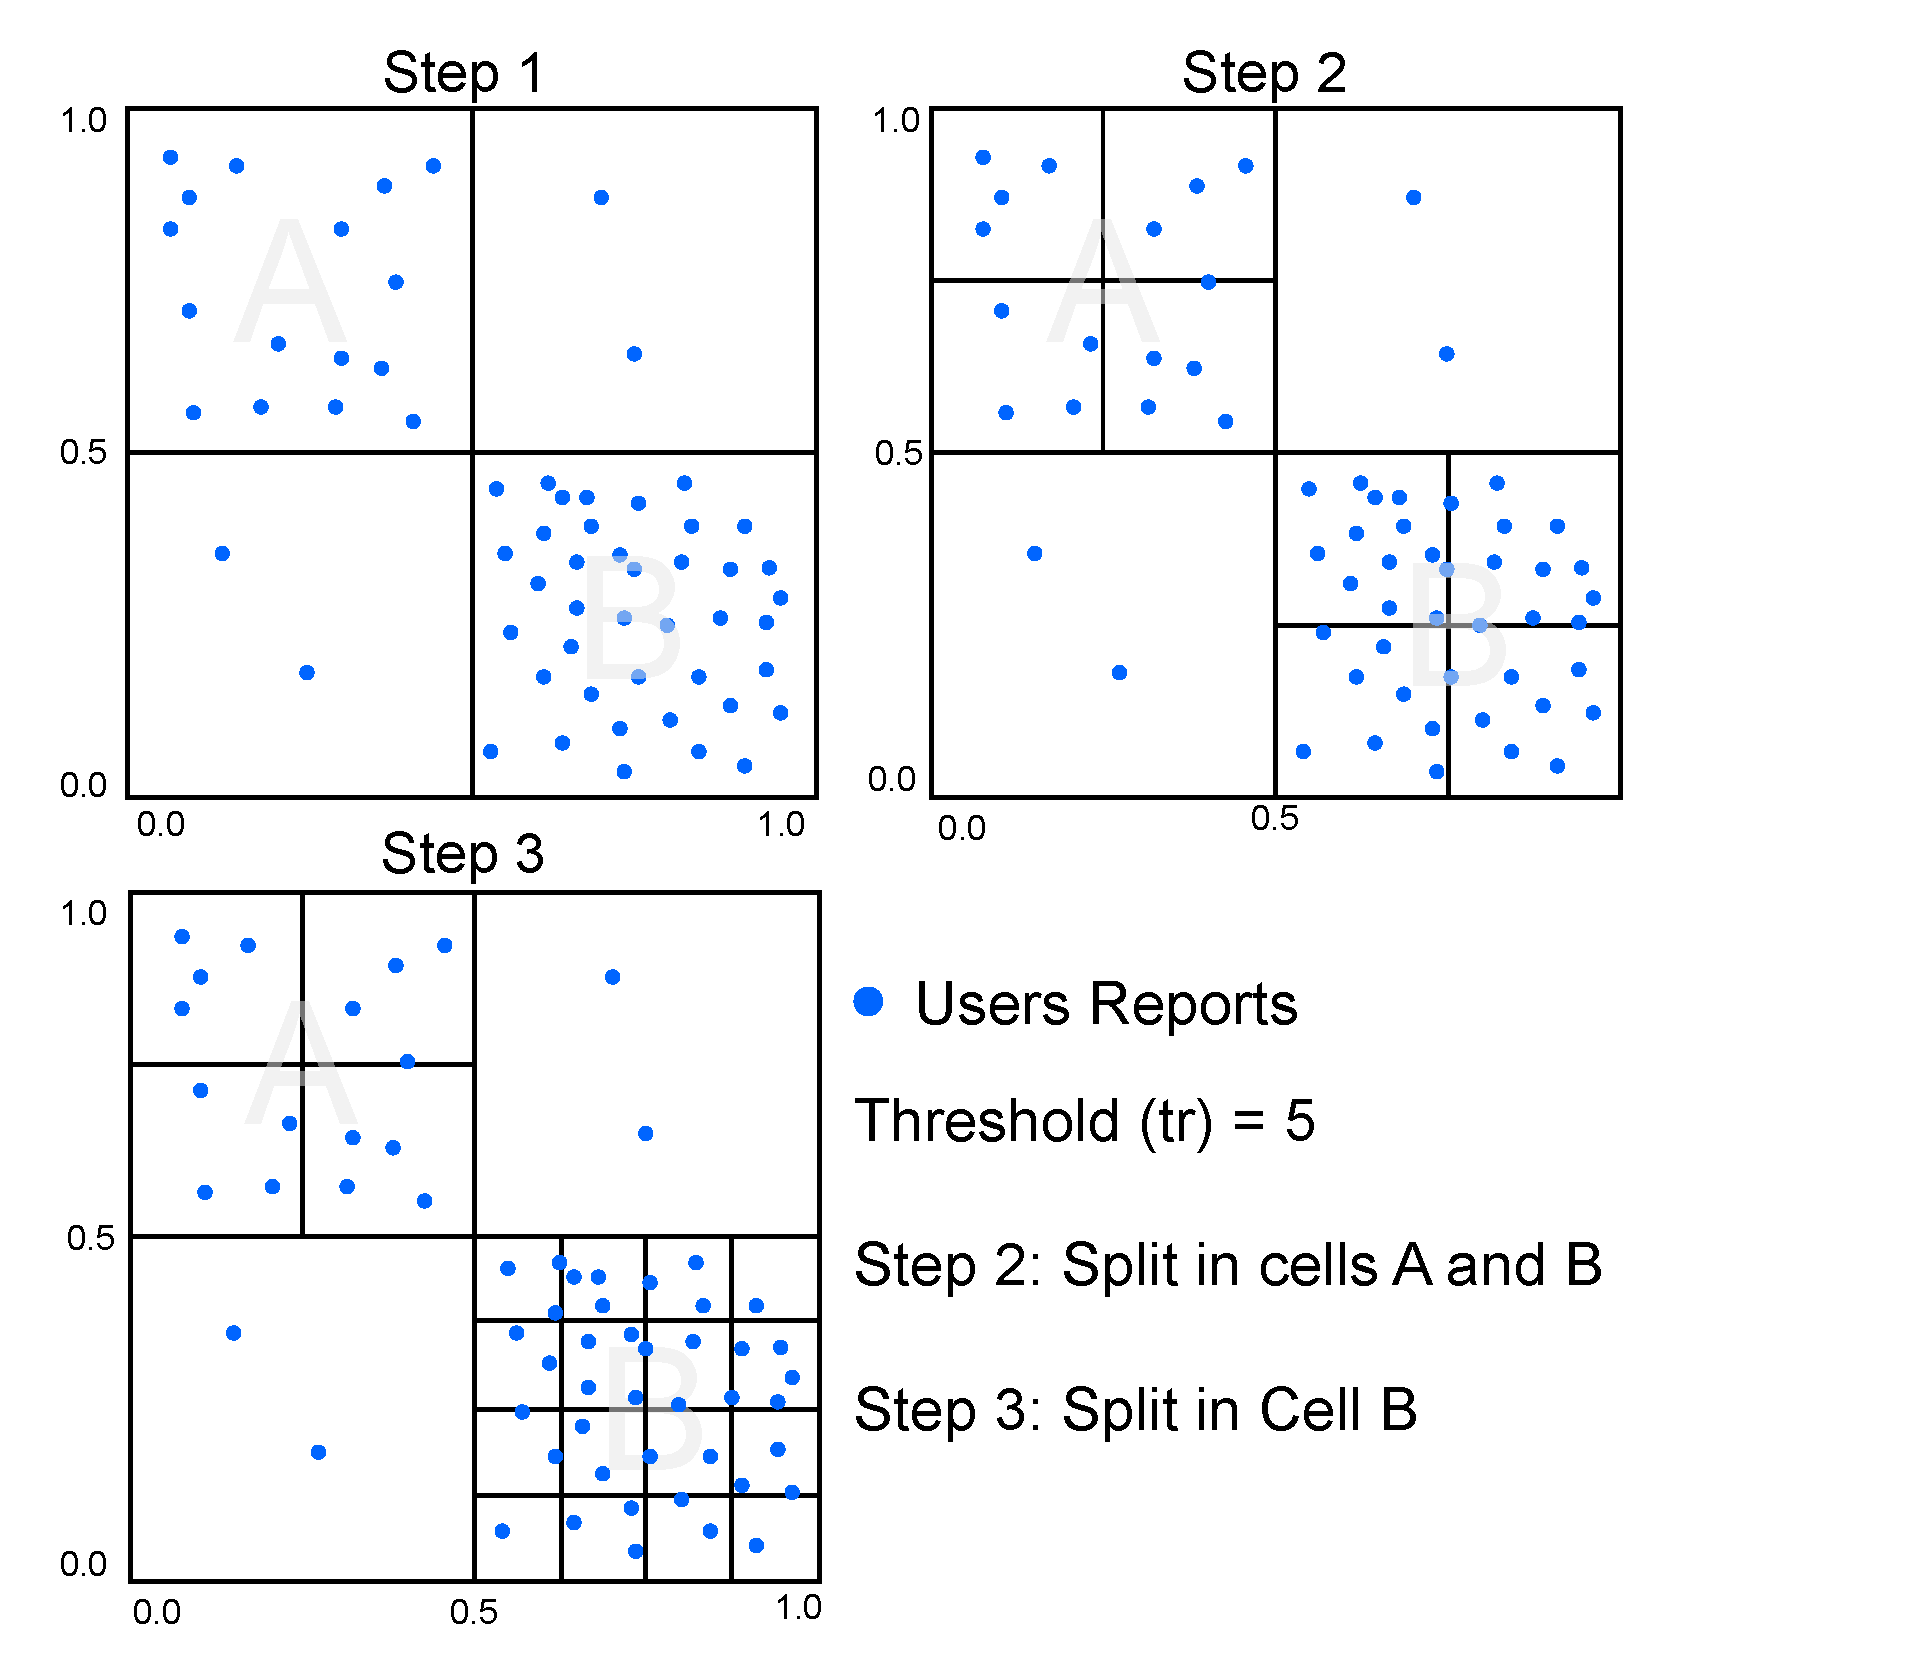
\includegraphics[width=\linewidth]{sections/figures/split_grid_seq_new.pdf}
    \caption{Illustration of the adaptive grid process: Cell A is split into four sub-cells after exceeding the threshold, and Cell B undergoes an additional split into sixteen sub-cells.
    }
    \label{fig:grid_adaptation}
\end{figure}

The first step in constructing the adaptive grid is to define the maximum allowable number of reports per cell, denoted as the cell threshold $tr$, which is determined by privacy requirements. Once the aggregator processes the users' reports for a specific timestamp $t$, it calculates the count $c_i$ of reports for each cell $g \in G$. Cells with report counts exceeding the threshold tr are recursively subdivided into four uniform cells, each occupying an equal portion of the original cell's spatial area. Subsequently, the count for each newly formed cell is assigned as one-quarter of the original cell count c, allowing the adaptive grid to dynamically adjust to areas of high report density by increasing granularity. This process is repeated until all cells satisfy the threshold tr. The complete algorithm for constructing the adaptive grid is detailed in Algorithm \ref{alg:recursive_adaptive_grid_creation}.

\begin{algorithm}[htb]
\small
\SetKwInOut{Input}{Input}
\SetKwInOut{Output}{Output}
\SetKwFunction{FGrid}{AdaptativeGrid}
\SetKwFunction{FSplit}{SplitCell}
\SetKwFunction{FMain}{Main}
\SetKwProg{Fn}{Function}{:}{}
\SetAlgoNoLine

\Input{Grid $G$, Estimated frequency for timestamp \( t \), Cell threshold \( tr \)}
\Output{Adaptive grid with updated cell counts}

\Fn{\FGrid($G$)}{
    % Process the frequency estimations to aggregate counts for each grid cell\;
    Calculate $\forall i\in G: c_i := \hat{f}_i$\;
    \For{each cell \( i \)}{
        SplitCell($\langle i, c_i\rangle$)\;
    }
}

\Fn{\FSplit($\langle i, c_i\rangle$)}{
    \If{\( c_i > tr \)}{
        Split cell \( i \) into four sub-cells of equal area\;
        \For{each sub-cell \( j \) of cell \( i \)}{
            Set count for sub-cell \( j \) to \( c_j = \frac{c_i}{4} \)\;
            \For{each cell \( i \)}{
                SplitCell($\langle i, c_i\rangle$)\;
                %Recursive call
            }
        }
    }
}
% \Return{Adaptive grid with updated cell counts}
\caption{Adaptive Grid Creation Algorithm}
\label{alg:recursive_adaptive_grid_creation}
\end{algorithm}
% 
Figure \ref{fig:grid_adaptation} illustrates the grid adaptation process. In the transition from Box 1 to Box 2, cells $A$ and $B$ are each split into four smaller cells. While cell $A$ reaches a count below the threshold $tr$, cell $B$ still exceeds the threshold, requiring an additional split in Box 3. As a result, all cells achieve a more balanced distribution of reports, ensuring a more uniform spatial representation. The time complexity of the adaptive grid creation is $\mathcal{O}(k \log n)$, where $k$ is the number of initial grid cells and $n$ is the number of user reports, reflecting the recursive subdivision of high-density cells.


\subsection{Frequency Estimator Framework}
\label{sec:fef}

ALOG comprises two main components: the users, who send encoded reports of their private locations, and the aggregator, who is responsible for collecting these reports and estimating the frequency of each grid cell. Beyond frequency estimation, the aggregator also contributes to generating and distributing the adaptive grid—a spatial representation that dynamically adjusts according to report density—to users. This adaptive grid enables refined spatial partitioning that is aligned with the population distribution, enhancing the precision of data collection and analysis.

Initially, the aggregator broadcasts a uniform grid accessible to all users, partitioning the reference space—such as a city—into square cells of equal size. On the user side, each user encodes their current location according to the grid provided by the aggregator, as detailed in Section \ref{sec:space_partition}. Utilizing a local differential privacy protocol, each user sends a noisy, obfuscated report of their location back to the aggregator. ALOG leverages the LOSUE protocol \ref{sec:losue}, which, following empirical analysis, has proven well-suited to this context; however, other longitudinal LDP protocols could also be employed.

Grid refinement is essential for reducing non-uniformity errors and improving data utility. However, evolving grids during anonymization can decrease memoization efficiency, leading to higher privacy budget consumption. This inefficiency arises because new cells are created with each new grid generated during the adaptation process. As a result, the previous canonical mapping of data to grid cells must be discarded, requiring the system to reinitialize the memoization for the newly created grid structure.

To mitigate this trade-off between budget consumption and grid adaptation, we propose a Grid Adaptation Window (GAW) mechanism. This mechanism ensures that grid adaptations occur only after every $w$ consecutive timestamps, after which the updated grid is broadcast to the users. Figure \ref{fig:window} illustrates the grid adaptation process with a window size of 2. Despite the use of GAW, the aggregator continues performing frequency estimations at each timestamp, ensuring continuous system monitoring and analysis. 

\begin{figure}[!ht]
    \centering
    \Description{GAW process}
    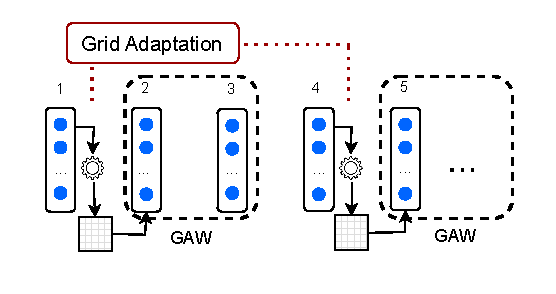
\includegraphics[width=0.8\linewidth]{sections/figures/gaw.pdf}
    \caption{GAW: Grid Adaptation Window mechanism with time window of size $w=2$}
    \label{fig:window}
\end{figure}

An additional benefit of the GAW is that it addresses situations where grid refinement is not always necessary. In some cases, the gain from refining the grid is not significant enough to justify the additional computational cost, as there may be little to no change between consecutive occurrences. In these situations, the GAW mechanism effectively reduces unnecessary grid adaptations, ensuring that system performance remains optimal without compromising the accuracy of the frequency oracles. The entire ALOG algorithm is detailed in Algorithm \ref{alg:alog_combined}.

% In the remainder of this section, we present a detailed exploration of the variations introduced by the proposed ALOG approach. The full ALOG algorithm is detailed in Algorithm \ref{alg:alog_combined}.


\begin{algorithm}[h]
\small
\SetKwInOut{Input}{Input}
\SetKwInOut{Output}{Output}
\SetAlgoNoLine

% User-side Algorithm
\textbf{User-side:} \\
\Input{$w$ \textit{(grid adaptation window)}}
\Output{Report $\hat{r}_i$}

\For{each timestamp $t$}{
    $l_i$ = Capture current location \\
    $G$ = Receive the Grid from Server\\
    $r_i$ = Encode($l_i$,$G$) \\
    $M$ = Initialize the Memoization Vector ($G$) \\

    $\hat{r}_i$ = LDP Protocol($r_i$, $G$, $M$)\;

    \If{\( t \% w == 0 \)}{
        $M$ = Initialize the Memoization Vector ($G$)\;
    }
}

% Server-side Algorithm
\textbf{Server-side:} \\
\Input{$tr$ \textit{(Cell Threshold)}, $w$ \textit{(grid adaptation window)}}
\Output{Adaptive grid, Frequency Estimations}

$G$ = Initialize the initial Grid\;

Process the reports to aggregate counts for each grid cell\;

\For{each timestamp $t$}{
    $R$ = Receive the reports for all users \\
    $F$ = Aggregate the reports to process the frequency estimation ($R$)\;
    \If{\( t \% w == 0 \)}{
        $G$ = Adaptive Grid Creation Algorithm ($G$, $F$, $tr$)\;
    }
}
\caption{ALOG Algorithm}
\label{alg:alog_combined}
\end{algorithm}

We propose three variations of the ALOG approach to determine the most effective solution for anonymizing user location reports in the context of grid refinement and data utility. The first variation, \textbf{ALOG-2R}, implements a two-round sanitization process designed to improve both grid refinement and the utility of the data. In the first round, each user $i$ anonymizes their location report using the initially provided uniform grid, allocating only a fraction of the available privacy budget to this step. For example, suppose a user $i$ has a true location at $(x_i, y_i)$, and the initially assigned grid cell is $g_0$. The user first encodes their location into the grid cell $g_0$ (e.g., by rounding their location to the nearest cell in the grid). The user then applies a Local Differential Privacy (LDP) protocol, utilizing a fraction of the total privacy budget to anonymize the encoded location. The resulting anonymized report, denoted as $\hat{r}_i$, is sent to the aggregator. This initial stage aims to provide a preliminary anonymized data sample to the aggregator.

Once the aggregator has collected the anonymized reports from all users, it proceeds to refine the spatial grid based on these reports. Specifically, the aggregator applies the Adaptive Grid Creation Algorithm (Algorithm \ref{alg:recursive_adaptive_grid_creation}) to construct a refined, adaptive grid that more accurately reflects the underlying data distribution. This adaptive grid is tailored to capture variations in the density of user locations, allowing for more precise spatial partitioning.

In the second round, the user $i$ now anonymizes their true location using the refined grid. For instance, if the user's true location $(x_i, y_i)$ falls in a newly created, smaller grid cell $g_1$ (which results from the adaptive grid refinement), the user will now encode their location into this smaller, more precise grid cell $g_1$. The user then applies the remaining portion of their privacy budget to anonymize the location in this refined grid cell, using the same LDP protocol as in the first stage. This refined anonymization ensures that the user's location is represented with higher precision according to the new adaptive grid. The anonymized report is then sent to the aggregator. After all users have submitted their second-round reports, the aggregator collects these updated anonymized reports and performs frequency estimation for the given timestamp. With grid refinement in the first stage and a more precise anonymization in the second stage, this two-stage process results in improved utility. By incorporating the adaptive grid refinement early on, ALOG-2R ensures that the data is processed with an optimized spatial partitioning, leading to more accurate frequency estimations while maintaining a strong privacy guarantee.

Alternatively, \textbf{ALOG-1R-a} (One-Round Sanitization — Adaptive) and \textbf{ALOG-1R-b} (One-Round Sanitization — Baseline) utilize a single-round sanitization process. In both variations, users initially report perturbed data using a uniform grid, and the adaptive grid is applied only in subsequent reports. The key distinction between ALOG-1R-a and ALOG-1R-b lies in the choice of the base grid used during the adaptation process.


In ALOG-1R-a, the base grid used for adaptation is not static. Instead, the grid from the previous adaptation step serves as the input for the Adaptive Grid Creation Algorithm. This allows for incremental refinements over time, where the grid is continuously adjusted to reflect the evolving spatial patterns of user locations. For instance, suppose in the first timestamp, a user $i$ has a true location at $(x_i, y_i)$, which initially maps to a grid cell $g_0$. After anonymizing the location using LDP and sending the anonymized data to the aggregator, the adaptive grid is refined based on the collected reports. When the user submits their report in the next timestamp, the adaptive grid generated from the prior stage is used as the base grid for further refinement. If the user's true location $(x_i, y_i)$ now falls into a more precise, smaller grid cell $g_1$ in this updated grid, the user will anonymize their location based on this refined grid, improving the accuracy of the spatial partitioning with each adaptation step. This dynamic approach allows the system to adapt to changing patterns in user data, improving the overall utility while maintaining privacy.

Conversely, in ALOG-1R-b, the algorithm takes a different approach. Here, the adaptive grid is reset at every adaptation step, and the algorithm consistently uses the default uniform grid as the base grid for every iteration of the grid refinement process. In each adaptation step, the algorithm ignores any previous refinements and starts from the uniform grid, applying the Adaptive Grid Creation Algorithm as if it were the first round of processing. For example, a user $i$'s true location $(x_i, y_i)$ is first mapped to a grid cell $g_0$ of the uniform grid. After anonymizing their location using LDP and sending the anonymized report to the aggregator, the grid is adapted based on the collected data. This new adaptive grid will be used in the next timestamp for users to anonymize their location, but the grid is discarded for the next adaptation process. When the user submits their second report, the algorithm again uses the uniform grid as the base for the refinement, disregarding the previous adaptation. This results in a stable reference framework for the grid adaptation process, which may be more predictable but does not account for changes in user spatial distributions over time.


% \begin{figure}[!ht]
%     \centering
%     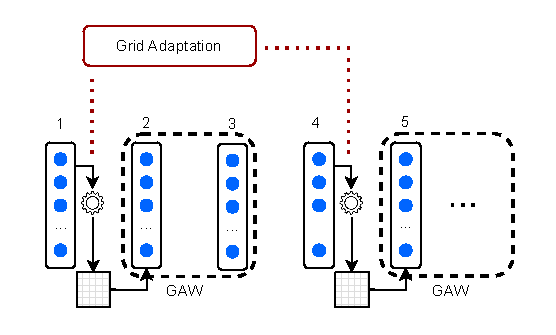
\includegraphics[width=0.8\linewidth]{sections/figures/ldpFE_trajectory-GAW.pdf}
%     \caption{GAW: Grid Adaptation Window mechanism with time window of size $w=2$}
%     \label{fig:window}
% \end{figure}


% \begin{table}[h!]
% \centering
% \caption{ALOG Variations}
% \footnotesize
% \begin{tabular}{l|c|c}
% % \begin{tabular}{ccc}
% \toprule
% \textbf{Approach} & \textbf{Rounds of Sanitization} & \textbf{Base Grid for Adaptation} \\
% \midrule
% ALOG-2R & Two-round & Previous Grid \\
% ALOG-1R-a & Single round & Previous Grid \\
% ALOG-1R-b & Single round & Uniform Grid \\
% \bottomrule
% \end{tabular}
% \end{table}

\begin{figure}[!ht]
    \centering
    \Description{Aloq workflow}
    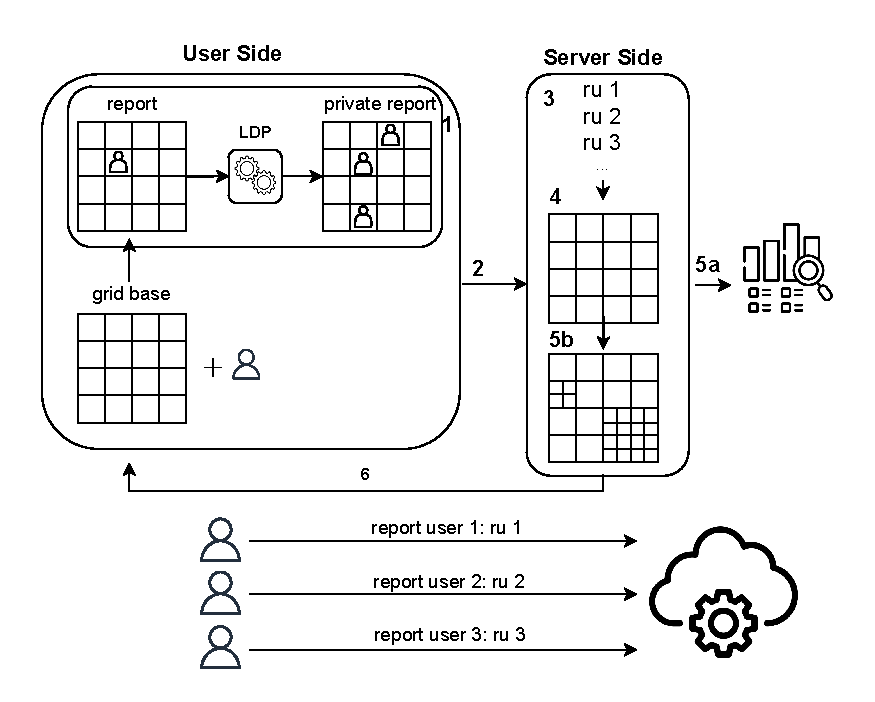
\includegraphics[width=0.8\linewidth]{sections/figures/alog_fe.pdf}
    \caption{ALOG Workflow - Step 1: Users sanitize their own reports. Step 2: Send the sanitized reports to the aggregator. Step 3: Aggregate received reports. Step 4: Process count for each cell. Step 5a: Perform frequency estimation. Step 5b: Grid adaptation to refine spatial granularity. Step 6: Broadcast the new Grid}

    \label{fig:alog_wf}
\end{figure}

The workflow of ALOG is illustrated in Figure \ref{fig:alog_wf}. The process begins with Step 1, performed on the user side, where each user encodes their location using the current base grid provided by the aggregator. This grid could either be the initial uniform grid (for ALOG-1R-b) or the refined grid from the previous moment (for ALOG-1R-a and ALOG-2R). The user applies a Local Differential Privacy (LDP) protocol to anonymize the location report in all approaches. Once anonymized, the report is transmitted securely to the aggregator, completing Step 2.

In Step 3, the aggregator collects all received reports. Step 4 follows, where the aggregator counts the occurrences within each grid cell to estimate the spatial distribution of user locations. Step 5a is executed at every timestamp, regardless of the approach. In this step, the aggregator publishes the estimated spatial distribution for each grid cell based on the received reports. This frequency estimation is critical for maintaining real-time monitoring of the data. The distinction arises when a Grid Adaptation Window (GAW) concludes. The GAW mechanism, primarily used in ALOG-2R and ALOG-1R-a, allows the grid adaptation process to occur only after a predefined number of timestamps (denoted as w). When this window ends, Step 5b is triggered. During Step 5b, the grid cells are adjusted based on report density. This refinement aims to enhance spatial resolution and precision, tailoring the grid to represent the underlying distribution of user locations better. This adjustment will occur as follows for each approach:
% 
\begin{itemize}
    \setlength{\parskip}{0pt}
    \setlength{\itemsep}{0pt plus 1pt}
    \item ALOG-2R: Grid refinement occurs after every w timestamp, allowing for dynamic, incremental adaptations. This means that after each window of w timestamps, the aggregator adapts the grid based on the spatial distribution observed in those reports.
    \item ALOG-1R-a: Similarly, the grid is adapted after every w timestamps, but in this approach, the refinement is based on the previously adapted grid. The grid evolves incrementally, becoming more precise with each new adaptation.
    \item ALOG-1R-b: In this approach, even when the GAW ends, the grid is reset to the initial uniform grid at every adaptation step, discarding any previous refinements. This provides a stable reference framework but does not consider previous grid adaptations.
\end{itemize}
% 
Finally, in Step 6, the aggregator broadcasts the refined grid back to the users. This ensures that users always work with an up-to-date spatial representation of the data. The users then continue the process of encoding, anonymizing, and sending reports based on the latest grid, ensuring that the system adapts to real-time patterns. \looseness=-1

This entire workflow is designed to repeat iteratively, maintaining a dynamic balance between spatial precision and privacy guarantees. The GAW ensures that grid adaptations occur controlled, reducing unnecessary overhead, while the different approaches (ALOG-1R-a, ALOG-1R-b, and ALOG-2R) offer flexibility depending on the need for stability versus dynamic adaptation.

On the client side, the ALOG algorithm \ref{alg:alog_combined} has a per-timestamp time and space complexity of $\mathcal{O}(k)$, where $k$ is the number of grid cells. This cost stems from encoding the location as a unary vector and applying the LDP mechanism. The time complexity of the ALOG algorithm on the server side, assuming a one-round approach, can be described in terms of the number of grid cells $k$, the number of user reports $n$, and the grid adaptation window size $w$. For each timestamp, the server processes $n$ reports and performs frequency estimation over $k$ cells, leading to a per-timestamp cost of $\mathcal{O}$($nk$). Every $w$ timestamps, the adaptive grid is updated using a recursive algorithm, whose worst-case cost is $\mathcal{O}(k \log n)$ due to cell subdivisions based on report density. Thus, over a time horizon $T$, the amortized server-side complexity becomes 
$\mathcal{O}$($Tnk + wTk\log n$), balancing continuous frequency estimation with periodic grid refinement.

\subsection{Privacy and Utility Analysis}
\label{sec:privacy}

In our approach, we employ LDP to protect user privacy while estimating the frequency of each grid cell in a spatial domain. Each user perturbs their location data locally before transmitting it to a centralized aggregator. This is done using the LOSUE protocol, as Section \ref{sec:losue} explains.

At each timestamp, ALOG uses at most a privacy budget of $\epsilon_\infty$, even ALOG-2R. In the case of ALOG-2R, the $\epsilon_\infty$ is divided across two stages: a fraction of $\epsilon_\infty$ is spent in the first stage, and the remaining fraction is applied in the second stage. Like other data collection models, whether using adaptive grids or not, ALOG consumes a privacy budget of $\epsilon_\infty$ for a single report, which is the single report's upper bound. 

Proposition \ref{prop:alogdp} provides a pessimistic worst-case privacy guarantee for our approach. Nevertheless, our experiments demonstrate that ALOG achieves Pareto efficiency -- a state where no further improvement can be made to one objective (e.g., utility) without degrading another (e.g., privacy) -- even with a slightly higher theoretical privacy budget than competing methods.
\newcommand{\budget}{\eta \epsilon_\infty}

\begin{proposition}[ALOG's Privacy Guarantee]
    The ALOG algorithm guarantees, in the worst case,  
    \(\budget\)-local differential privacy, where: \looseness=-1
        \(\eta = \left( \sum_{r=0}^R (k - \bar{k}) \cdot 4^r + \bar{k} \right)\),
        \( \bar{k} \) is the number of initial grid cells satisfying the threshold condition,
        \( R = \left\lceil \log_4 \frac{|U|}{tr} \right\rceil \) is the maximum recursion depth of the Algorithm \ref{alg:recursive_adaptive_grid_creation},
        \( \epsilon_\infty \) is the per-report privacy budget under \( \Psi \), the underlying LDP mechanism.  
    \label{prop:alogdp}
\end{proposition}
\begin{proof}
    At initialization, the grid contains \( k \) cells, of which \( \bar{k} \) satisfy the threshold \( tr \). The remaining \( k - \bar{k} \) cells are recursively split (at most \( R \) times) until all subcells meet \( tr \), as formalized in Algorithm \ref{alg:recursive_adaptive_grid_creation}. \looseness=-1
    For recursion level \( r \in [0, R] \), the grid contains \( (k - \bar{k}) \cdot 4^r + \bar{k} \) cells. Summing over all levels, the \textit{total cumulative cell count} is:  
    \( 
    \sum_{r=0}^R \left( (k - \bar{k}) \cdot 4^r + \bar{k} \right).  
    \) 
    Since each user’s location report is privatized via \( \Psi \) (an \( \epsilon_\infty \)-LDP protocol), the \textit{longitudinal privacy cost} of ALOG, accounting for adaptive grid construction and repeated reporting, is bounded by the worst-case total cell count multiplied by \( \epsilon_\infty \). This holds because:
    \begin{enumerate}
        \item \textit{User-side perturbation}: Each report is independently \( \epsilon_\infty \)-LDP.
        \item \textit{Aggregator-side adaptation}: The grid’s dynamic refinement does not access raw data, relying only on privatized counts.
    \end{enumerate}
    The total cumulative cell count reflects the worst-case scenario where Algorithm \ref{alg:recursive_adaptive_grid_creation} exhausts all possible recursions. Each cell is sanitized only once during the longitudinal process by employing memoization in the LDP protocol. Thus, since the upper bound on cell count is \( \eta \), the maximum number of sanitizations is precisely the cumulative cell count.
    As each report is independently \( \epsilon_\infty \)-LDP and there are at most \(\eta\) cells in the grid, our proposed algorithm is \(\budget\)-local differentially private.
\end{proof}


In ALOG, both the frequency estimation (Section \ref{sec:freq_estimator}) and grid adaptation (Section \ref{sec:adaptative_grid}) processes operate on the perturbed reports, ensuring that individual location data remains protected. As Proposition \ref{prop:seq_processing} states, any function applied to the output of an $\epsilon$-LDP mechanism preserves $\epsilon$-LDP privacy guarantees, meaning that the privacy established by the initial LDP perturbation is maintained throughout these post-processing steps without introducing additional privacy risks.

The granularity of the initial grid used in LDP significantly impacts data sensitivity and privacy preservation. This relationship is analyzed through variance, a key measure of frequency estimate accuracy and reliability. The variance of LDP protocols is inversely proportional to the number of times a value \(v_i\) has been reported \cite{arcolezi2022frequency}, meaning that higher variance indicates greater uncertainty and error in estimates. In comparison, lower variance suggests more accurate results. Fine-grained grids yield fewer reports per cell in low-density areas, increasing variance and making estimates less reliable. Conversely, in high-density areas, fine-grained grids can maintain utility without compromising privacy, as the number of reports per cell remains high, reducing variance.

ALOG directly addresses the variance problem by using coarser grids in low-density areas, increasing reports per cell and decreasing variance. ALOG refines the grid in high-density areas to maintain utility, and the higher density helps control variance. Due to this adaptive behavior, ALOG's grids tend to keep the density between cells close to uniformity, further enhancing the accuracy of estimates while preserving privacy.

When handling longitudinal data, ALOG mitigates privacy loss through the Grid Adaptation Window (GAW). By regulating the frequency of grid adjustments, the GAW ensures that the grid adapts only after every \(w\) timestamps, limiting the reinitialization of memorization, which is a process that consumes the privacy budget. This mechanism balances the utility gains offered by dynamic grid adaptation and the potential increase in privacy loss resulting from frequent re-randomization, thus maintaining privacy protection while enhancing utility.